\section{Quantum Physics Basics and the Stern-Gerlach Experiment}
Some of the key features of quantum physics are exhibited in the Stern-Gerlach experiment (see figure \ref{stern}).
In this experiment, silver atoms are heated in a furnace which randomly emerge from the furnace with various velocities. By aligning two plates with circular holes near the furnace, it is possible to select a subset of the emerging silver atoms having (approximately) the same momentum\footnote{The \emph{momentum}\index{momentum} of an atom is its mass multiplied by its velocity. See footnote \ref{Velocityfootnote} on page \pageref{Velocityfootnote} for a definition of velocity.} to form a beam in one direction, the other silver atoms having been absorbed by the two plates. This beam of silver atoms is then directed between two magnets with the north pole of one magnet being aligned toward the south pole of the other magnet as shown in figure \ref{stern}.
\begin{figure}[ht!]
\captionsetup{justification=justified}
\centering
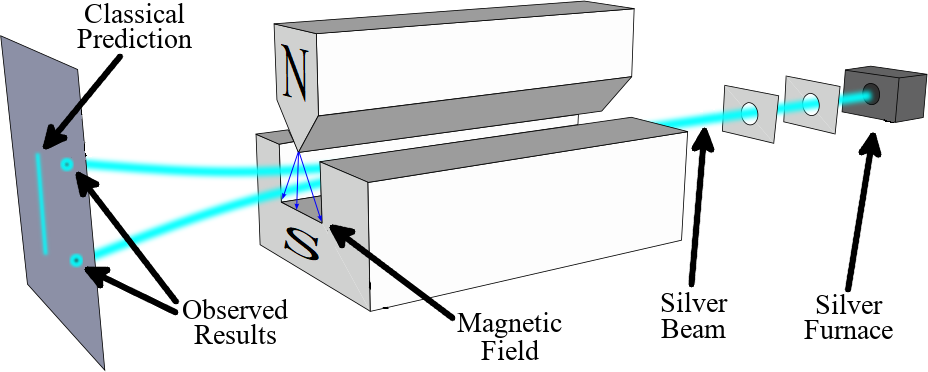
\includegraphics[width=100mm]{Chapter01/Stern-Gerlach_experiment_svg.png}
\caption[Stern-Gerlach Experiment]{The Stern-Gerlach Experiment.\protect\footnotemark}
\label{stern}
\end{figure}
\footnotetext{ Original diagram drawn by Theresa Knott. Labeling was modified for use in this dissertation. This image is licensed under the Creative Commons Attribution-Share Alike 4.0 International license. Source: https://commons.wikimedia.org/wiki/File:Stern-Gerlach\_experiment\_svg.svg.}
Now silver atoms have a property somewhat analogous to the classical notion of \emph{angular momentum}\index{angular momentum}. For instance, a spinning top has angular momentum as shown in figure \ref{spintop}. Angular momentum is a \emph{vector}\index{vector}, that is, it has direction and magnitude. In the case of a spinning top, the direction of the angular momentum would be parallel to the axis of rotation, pointing one way or the other depending on whether the rotation was clockwise or counterclockwise. The magnitude of the angular momentum would then be proportional to the \emph{angular velocity}\index{angular velocity} of the spinning top, so that the faster the top was spinning, the greater the angular velocity would be, and hence, the greater the angular momentum would be.
\begin{figure}[ht!]
\captionsetup{justification=centering}
\centering
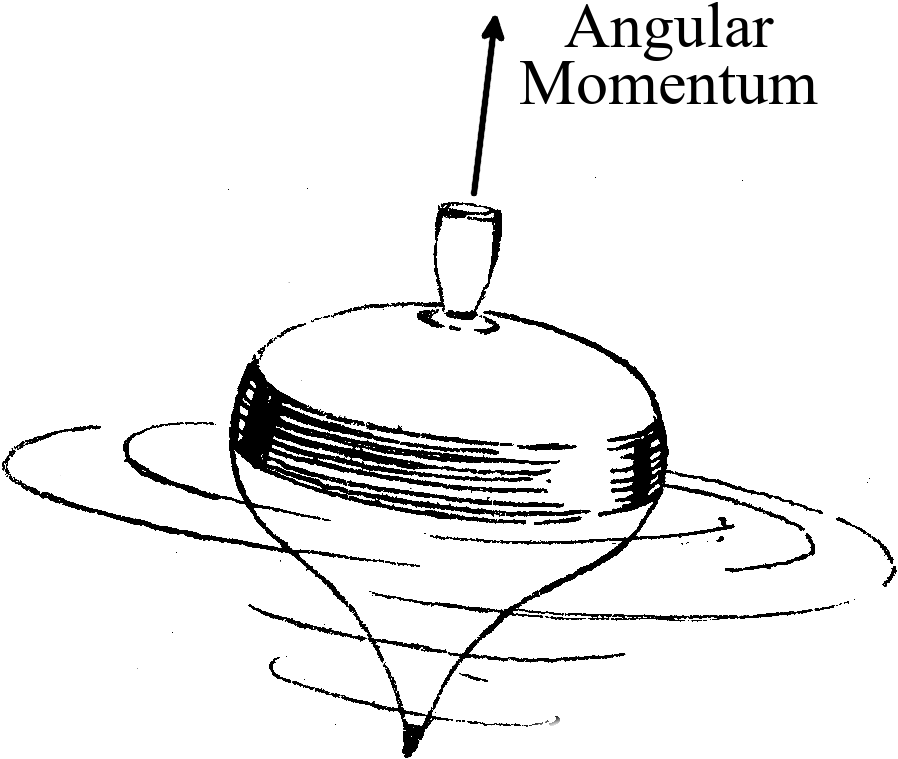
\includegraphics[width=50mm]{Chapter01/Top_(PSF)2.png}
\caption[Angular Momentum of a Spinning Top]{Angular Momentum of a Spinning Top.\protect\footnotemark}
\label{spintop}
\end{figure}

Now if we tried to understand the angular momentum of a silver atom classically, we would expect the magnetic field of the two magnets to interact with the silver atom in a way that was determined by the relative direction of the silver atom's angular momentum compared to the direction of the magnetic field. Since we would expect the silver atom to have an entirely random angular momentum, we would expect it to be deflected by varying degrees either up or down in the direction of the magnetic field. Thus, if a detection screen were placed beyond the two magnets which the silver atoms would hit, we would expect there to be a whole continuum of possible locations where the silver atoms would be detected. However, in reality, it is found that there are precisely two locations where the silver atoms hit the screen. It is as though the particles can spin either clockwise or anticlockwise, but that there is absolutely no variance in the angular speed at which they rotate. This is surprising. The angular momentum appears to be \textbf{quantized}\index{qunatization} in one of two directions, either parallel to the magnetic field or antiparallel\footnotetext{Drawing by Pearson Scott Foresman, Public domain, via Wikimedia Commons. Labeling was added for use in this dissertation. Original: https://commons.wikimedia.org/wiki/
File:Top\_(PSF).png.} to it.\footnote{See figure \ref{antiparallel} for what is meant be antiparallel.} Corresponding to this quantization of angular momentum, we say that the atom is either in the spin up state or the spin down state with respect to the direction of the magnetic field. 
\begin{figure}[ht!]
\captionsetup{justification=centering}
\centering
\fbox{\begin{picture}(65,50)
   \put(0,10){\vector(1,1){30}} %% a
   \put(5,25){$\vec{a}$}

   \put(65,40){\vector(-1,-1){30}} %% -a
   \put(30,25){$-\vec{a}$}
\end{picture}}
\vspace*{10px}
\caption[Meaning of antiparallel]{Meaning of antiparallel: the arrows in opposite directions are said to be antiparallel to one another.}\label{antiparallel}
\end{figure}\\
\noindent If the direction of the magnetic field is implicitly understood, we write $\ket*{+}$ and $\ket*{-}$ for the spin up and spin down states of the atom respectively. We refer to the symbols $\ket*{+}$ %
\nomenclature{$\ket*{+}$}{Generic spin up state, \nomrefpage}%
and $\ket*{-}$ %
\nomenclature{$\ket*{-}$}{Generic spin down state, \nomrefpage}%
as \textbf{ket-vectors}\index{ket-vector}, or simply as kets. We can think of the ket $\ket*{+}$ for instance as shorthand for the proposition “the particle is in the spin up state.” If we knew this proposition to be true, we would know which of the two locations on the detection screen the particle would end up if it were to travel between the two magnets of the Stern-Gerlach apparatus. If we need to specify the spin with respect to a particular direction of the magnetic field, say in the $\uvb{a}$-direction, %
\nomenclature{$\uvb{a}$}{Unit vector in a particular direction, \nomrefpage}%
 we write the corresponding spin up and down states as $\ket*{\uvbp{a}}$ %
\nomenclature{$\ket*{\uvbp{a}}$}{Spin up state in the $\uvb{a}$-direction, \nomrefpage}%
and $\ket*{\uvbm{a}}$. %
\nomenclature{$\ket*{\uvbm{a}}$}{Spin down state in the $\uvb{a}$-direction, \nomrefpage}%
For convenience, we write $\uvbp{a}$ %
\nomenclature{$\uvbp{a}$}{The location a particle in the state $\ket*{\uvbp{a}}$ would hit the detection screen, \nomrefpage}%
and $\uvbm{a}$ %
\nomenclature{$\uvbm{a}$}{The location a particle in the state $\ket*{\uvbm{a}}$ would hit the detection screen, \nomrefpage}%
respectively for the location that the particle would hit the detection screen.  

The question then arises as to what happens when we rotate the magnetic field around the axis of the particle beam in the Stern-Gerlach experimental setup. It turns out that when we do this, the atoms are again detected in only one of two locations (see figure \ref{rotate}).
\begin{figure}[ht!]
\captionsetup{justification=justified}
\centering
\usetikzlibrary {angles, quotes, calc} 
\pgfmathsetmacro{\ang}{-20}
\begin{tikzpicture}
\tikzset{
mydot/.pic={\fill (0,0) circle (\dotsize);}}
\coordinate (a) at (0, -2.1);
\coordinate (b) at (0, 2.1);
\coordinate (o) at (0, 0);
\coordinate (c) at ($ (o)!1! \ang:(a) $);
\coordinate (d) at ($ (o)!1! \ang:(b) $);
\draw (-5, -3) rectangle (5, 3);
\draw[thick, loosely dashed]  (d) pic {mydot} node[anchor=south west]{$\uvbp{b}$} -- (o) -- (b) pic {mydot} node[anchor=south ]{$\uvbp{a}$} pic [draw=black!50!black, solid, fill=black!10, angle radius=15mm, "$\theta$"] {angle = d--o--b}; 
\draw[thick, loosely dashed] (a) pic {mydot} node[anchor=north ]{$\uvbm{a}$} -- (o) -- (c) pic {mydot} pic {mydot} node[anchor= east]{$\uvbm{b}$};
\fill (o) circle (\dotsize);

\draw[thick, solid, -stealth] (-2,0) -- (-0.2,0);
\node[text width=2cm, align=center] at (-3.2,0) {\footnotesize Beam center  of  the  silver atoms};
\node[draw] at (3,-2){Detection Screen};
\end{tikzpicture}
\vspace*{10px}
\caption[Locations of detections on detection screen]{Locations of detections before and after rotating the magnetic field by an angle $\theta$. Before rotation, the particles can be detected at either location $\uvbp{a}$ or location $\uvbm{a}$. After the rotation, particles can be detected at either location $\uvbp{b}$ or $\uvbm{b}$. }
\label{rotate}
\end{figure}
\\ \noindent
So suppose we knew the particle was in a spin state such that it was on course to arrive at location $\uvbp{a}$ because we had previously directed it through another magnetic field in the $\uvb{a}$-direction. For example, see figure \ref{knownspin} for how this might be done.
\begin{figure}[ht!]
\captionsetup{justification=centering}
\centering
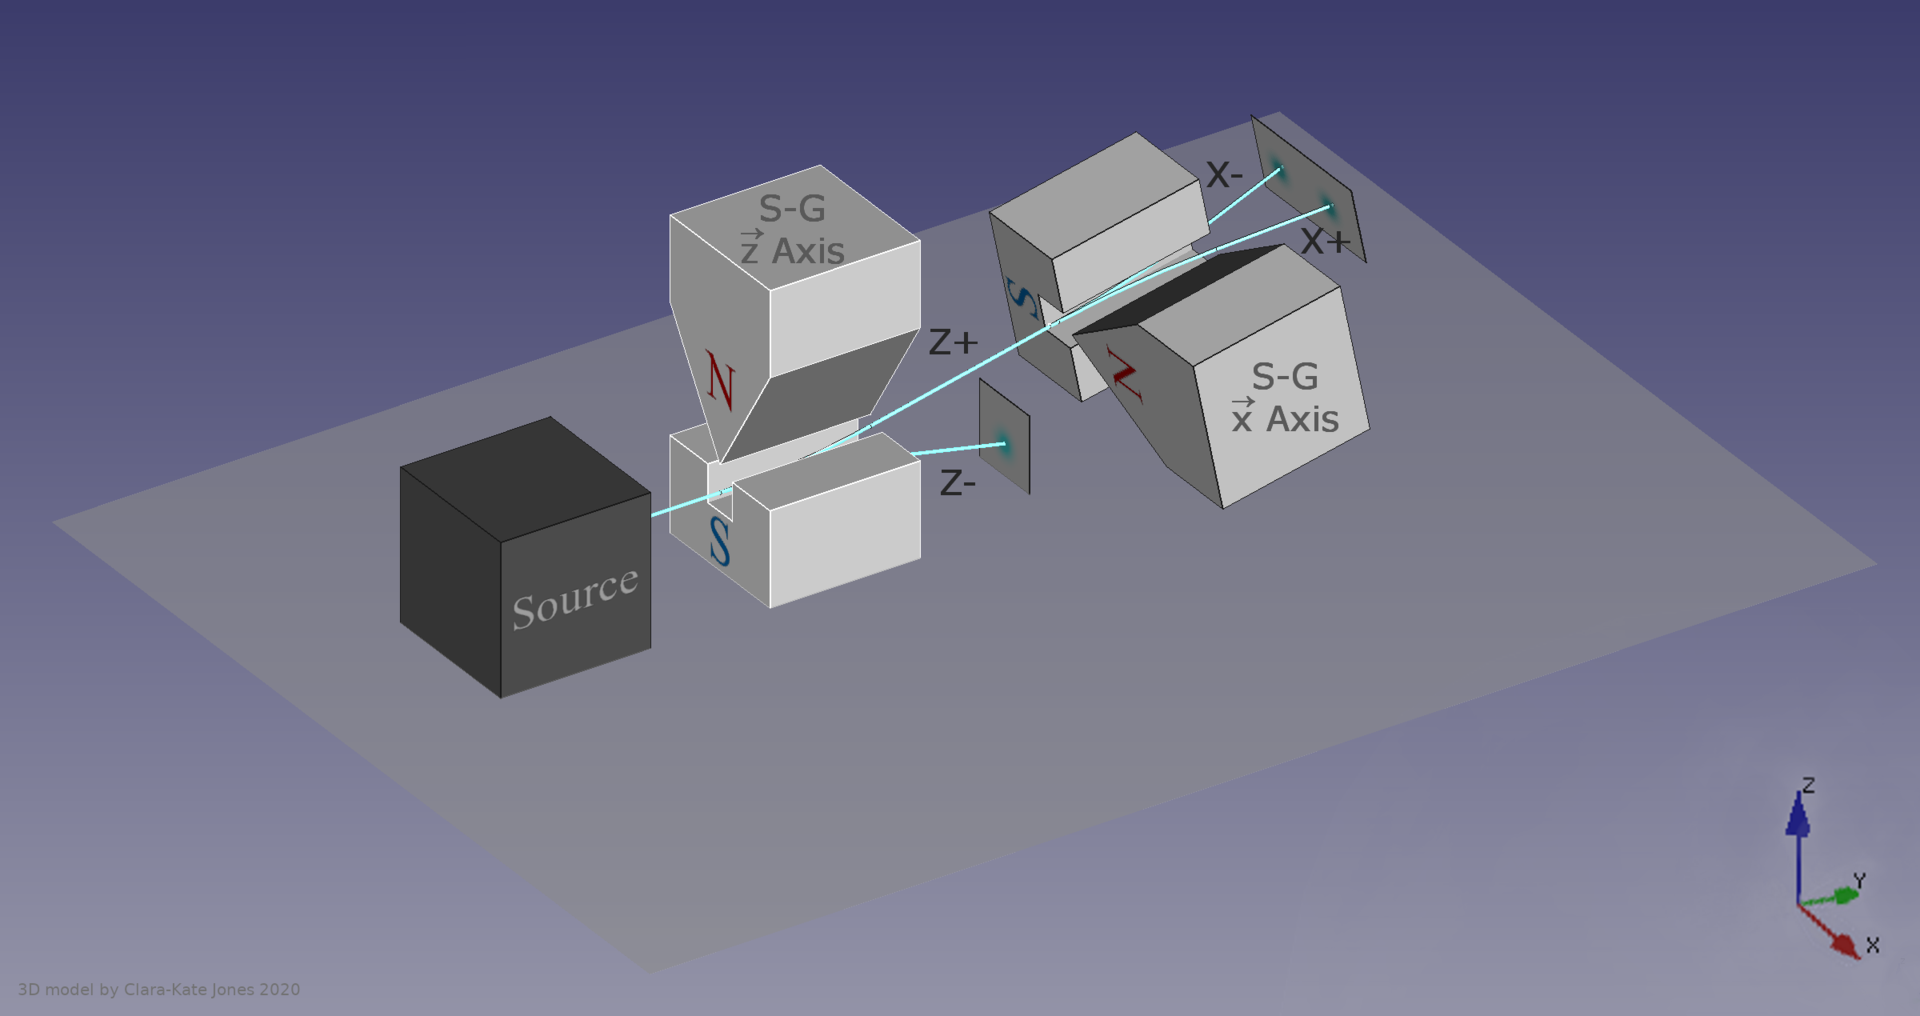
\includegraphics[width=100mm]{Chapter01/1920px-Stern-Gerlach_Analyzer_Sequential_Series_E2v.png}
\vspace*{10px}
\caption[Two Stern-Gerlach experiments in sequence]{Two Stern-Gerlach experiments in sequence. By directing the beam of particles through one magnetic field first, the particles emerging in one of the two beams will be in a known spin state before they enter the second magnetic field.\protect\footnotemark}
\label{knownspin}
\end{figure}
\footnotetext{Diagram by MJasK. This file is licensed under the Creative Commons Attribution-Share Alike 4.0 International license. Source: https://commons.wikimedia.org/wiki/File:Stern-Gerlach\_Analyzer\_Sequential\_Series\_E2.png. } In this experimental setup, the second magnetic field has been rotated by an angle of $90^\circ$ with respect to the first magnetic field. But suppose we just rotated the second magnetic field by a very small angle $\theta$ with respect to the first magnetic field. Then we would expect the particle now to arrive at a location  $\uvbp{b}$ close by to $\uvbp{a}$ as shown in figure \ref{rotate}. And this is what we notice experimentally for the most part. However, occasionally, the particle will arrive at location $\uvbm{b}$. The frequency of this occurrence becomes less and less the less and less the magnetic field is rotated (i.e. the smaller $\theta$ is), so that if the magnetic field is not rotated at all, i.e. $\theta=0$, the particle will always arrive at location $\uvbp{a}$. 
To capture the probabilistic nature of these outcomes, we use the bra-ket notation. Thus, if $\ket*{\psi}$ stands for either the $\ket*{\uvbp{a}}$ or the $\ket*{\uvbm{a}}$-state, and $\ket*{\chi}$ stands for either the $\ket*{\uvbp{b}}$ or the $\ket*{\uvbp{b}}$-state, then we define the bra-ket $\ip*{\psi}{\chi}\in\mathbb{C}$  %
\nomenclature{$\ip*{\psi}{\chi}$}{The bra-ket of two states $\ket*{\psi}$ and $\ket*{\chi}$, \nomrefpage} %
to be a complex number\footnote{Regarding the set of complex numbers $\mathbb{C}$, %
\nomenclature{$\mathbb{C}$}{The set of complex numbers, \nomrefpage}%
we will use the notation $i=\sqrt{-1}$. %
\nomenclature{$i$}{The square root of $-1$, $\sqrt{-1}$, \nomrefpage}%
Complex conjugation will be denoted by an overline so that $\overline{x+iy}=x-iy$ %
\nomenclature{$\overline{z}$}{The complex conjugate of a complex number $z$, \nomrefpage}% 
for real numbers $x$ and $y$. The modulus of a complex number $z=x+iy$ will then be given by $\abs{z}=\sqrt{z\overline{z}}=\sqrt{x^2+y^2}.$ %
\nomenclature{$\abs{z}$}{The magnitude of the complex number $z$, \nomrefpage}%
Since the defining property of  $\ip*{\psi}{\chi}$ is that $\abs*{\ip*{\psi}{\chi}}^2$ is the probability that the particle will be found to be in state $\ket*{\psi}$ given that we know that the particle is in state $\ket*{\chi}$, we have to choose an arbitrary phase to fully determine $\ip*{\psi}{\chi}$. } that satisfies the \textbf{Born Rule}\index{Born Rule},\label{bornrule} namely the rule that $\abs*{\ip*{\psi}{\chi}}^2$ is the probability that the particle will be found to be in state $\ket*{\psi}$ given that we know that the particle is in state $\ket*{\chi}$. For example, if $\abs*{\ip*{\psi}{\chi}}^2=\frac{1}{4},$ and we performed the experiment a thousand times with the particle initially prepared in the $\ket*{\chi}$-state, then we would expect the particle to be found in the $\ket*{\psi}$-state in around 250 runs of the experiment. Given the Born Rule, we  would thus expect $\abs*{\ip*{\uvbm{a}}{\uvbp{a}}}^2$ to be $0$, from which it will follow that $\ip*{\uvbm{a}}{\uvbp{a}}$ has to be $0$. The Born Rule also implies that $\abs*{\ip*{\uvbp{a}}{\uvbp{a}}}^2=1$. We will also insist that $\ip{\psi}{\chi}=\overline{\ip{\chi}{\psi}}$,\footnote{Note that this condition implies time symmetry: the probability a particle transitions from a state $\ket*{\chi}$ to a state $\ket*{\psi}$ will be the same as the probability a particle transitions from the state $\ket*{\psi}$ to the state $\ket*{\chi}$. This is in accord with the observation that closed quantum systems are symmetric on time-reversal. A more precise formulation of this statement is given by the CPT theorem e.g. see \cite[244]{WeinbergSteven1995Tqto}. This might at first seem surprising in the light of the fact that phenomena such as radioactive decay are not obviously time-symmetric. However, it turns out that this time asymmetry results from the quantum system not being closed. For more details, see \cite{Pascazio2013}.}  from which it will follow that $\ip*{\uvbp{a}}{\uvbp{a}}$ is a real number of modulus $1$ (i.e. $+1$ or $-1$). By convention, we choose $\ip*{\psi}{\chi}$  such that $\ip*{\psi}{\psi}$ is a real and positive number, in which case we must have $\ip*{\uvbp{a}}{\uvbp{a}}=1$.
If we now rotate the magnetic field by an angle $\theta$ as indicated in figure \ref{rotate}, the particle will be detected either at location $\uvbp{b}$ or location $\uvbm{b}$. We can then ask the question “given that the particle is in state $\ket*{\uvbp{a}}$, what is the probability that the particle will be found to be in state $\ket*{\uvbp{b}}$?” According to the notation discussed above, this probability will be $|\ip*{\uvbp{b}}{\uvbp{a}}|^2$ where $\ip*{\uvbp{b}}{\uvbp{a}}$ is a complex number such that $\ip*{\uvbp{b}}{\uvbp{a}}=1$ when $\theta =0$ and $\ip*{\uvbp{b}}{\uvbp{a}}=0$ when $\theta=180\degree.$ We would likewise expect $\ip*{\uvbp{b}}{\uvbm{a}}=0$ when $\theta =0$ and $\ip*{\uvbp{b}}{\uvbm{a}}=1$ when $\theta=180\degree.$ Since $\cos 0\degree = \sin 90\degree = 1$ and $\cos 90\degree = \sin 0\degree = 0$, we might guess that in general $\abs*{\ip*{\uvbp{b}}{\uvbp{a}}}=\abs*{\cos(\theta/2)}$ and  $\abs*{\ip*{\uvbp{b}}{\uvbm{a}}}=\abs*{\sin(\theta/2)}.$\footnote{Besides this guess being correct for angles such as $0\degree$ and $180\degree$, a further reason for thinking this is a good guess follows from the fact that since a particle in the $\ket*{\uvbp{b}}$-state must be measured to be  in either the $\ket*{\uvbp{a}}$-state or the $\ket*{\uvbm{a}}$-state when measured along the $\uvb{a}$-axes, from the Born Rule we must have 
$$ \abs*{\ip*{\uvbp{b}}{\uvbp{a}}}^2+\abs*{\ip*{\uvbp{b}}{\uvbm{a}}}^2=1.$$
But for any angle $\theta$ we also have 
$$\abs*{\cos(\theta/2)}^2+\abs*{\sin(\theta/2)}^2=1,$$
and so setting $\abs*{\ip*{\uvbp{b}}{\uvbp{a}}}=\abs*{\cos(\theta/2)}$
and  $\abs*{\ip*{\uvbp{b}}{\uvbm{a}}}=\abs*{\sin(\theta/2)}$
is consistent with these two equations.} 
Experimentation shows us that this guess is correct.
This suggests that we can express the state $\ket*{\uvbp{b}}$ in terms of the states $\ket*{\uvbp{a}}$ and $\ket*{\uvbm{a}}$. We thus suppose that 
\begin{subequations}\label{vectoradd}
\begin{align}
\ket*{\uvbp{b}}&=\alpha\ket*{\uvbp{a}}+\beta\ket*{\uvbm{a}}\label{vectoradd1}\\
\ket*{\uvbm{b}}&=\bar{\alpha}\ket*{\uvbm{a}}-\bar{\beta}\ket*{\uvbp{a}}\label{vectoradd2}
\end{align} 
\end{subequations}
for complex numbers $\alpha, \beta \in \mathbb{C}$ such that $|\alpha|^2+|\beta|^2=1$, and we suppose that the bra-ket has the \textbf{linearity}\index{linearity}\label{linearity} property so that  $\ip*{\psi}{\uvbp{b}}=\alpha\ip*{\psi}{\uvbp{a}}+\beta\ip*{\psi}{\uvbm{a}}$ and $\ip*{\psi}{\uvbm{b}}=\bar{\alpha}\ip*{\psi}{\uvbm{a}}-\bar{\beta}\ip*{\psi}{\uvbp{a}}$ for any state $\ket*{\psi}$. Then  it will follow that  $\ip*{\uvbp{b}}{\uvbm{b}}=0,$\footnote{To see this, by putting $\ket*{\psi}=\ket*{\uvbp{b}}$, we will have $\ip*{\uvbp{b}}{\uvbm{b}}=\bar{\alpha}\ip*{\uvbp{b}}{\uvbm{a}}-\bar{\beta}\ip*{\uvbp{b}}{\uvbp{a}}$ by equation (\ref{vectoradd2}). Since  $\ip*{\uvbp{b}}{\uvbm{a}}=\overline{\ip*{\uvbm{a}}{\uvbp{b}}}$ we have $\ip*{\uvbp{b}}{\uvbm{a}}=\bar{\beta}$ by equation (\ref{vectoradd1}), and likewise, since $\ip*{\uvbp{b}}{\uvbp{a}}=\overline{\ip*{\uvbp{a}}{\uvbp{b}}}$, we have $\ip*{\uvbp{b}}{\uvbp{a}}=\bar{\alpha}.$  Therefore,  $\ip*{\uvbp{b}}{\uvbm{b}}=\overline{\alpha}\overline{\beta}-\overline{\beta}{\overline{\alpha}}=0.$}  and that $\ip*{\uvbp{b}}{\uvbp{b}}=\ip*{\uvbm{b}}{\uvbm{b}} = 1.$\footnote{To see this, by putting $\ket*{\psi}=\ket*{\uvbp{b}}$ and using equation (\ref{vectoradd1}), we will have $\ip*{\uvbp{b}}{\uvbp{b}}=\alpha\ip*{\uvbp{b}}{\uvbp{a}}+\beta\ip*{\uvbp{b}}{\uvbm{a}}=\alpha\overline{\alpha}+\beta\overline{\beta}=\abs{\alpha}^2+\abs{\beta}^2=1.$ By a similar calculation, we also see $\ip*{\uvbp{b}}{\uvbp{b}}=1$.}  
If we then put  $\alpha=\cos(\theta/2)$ and $\beta=\sin(\theta/2)$, it will follow that $\abs*{\ip*{\uvbp{b}}{\uvbp{a}}}=\abs*{\cos(\theta/2)}$ and  $\abs*{\ip*{\uvbp{b}}{\uvbm{a}}}=\abs*{\sin(\theta/2)},$\footnote{To satisfy these criteria, $\alpha$ and $\beta$ are only determined up to rotation by a complex number. Rotating a complex number $z\in\mathbb{C}$ just means multiplying it by a complex number $\lambda$ of modulus $1$ (i.e. $\abs{\lambda}=1$) to get $\lambda z$. We would need to take into account this rotation factor if we considered the three-dimensional situation. Then, without loss of generality, $\alpha=\cos(\theta/2)$ and $\beta=e^{i\phi}\sin(\theta/2)$ where $\theta$ and $\phi$ are the polar and azimuthal angles respectively.} and so with these values for $\alpha$ and $\beta$ we will have
\begin{subequations}\label{spintrans}
\begin{align}
\ket*{\uvbp{b}}&= \cos(\theta/2)\ket*{\uvbp{a}}+\sin(\theta/2) \ket*{\uvbm{a}},\label{spintrans1}\\
\ket*{\uvbm{b}}&= \cos(\theta/2)\ket*{\uvbm{a}}-\sin(\theta/2) \ket*{\uvbp{a}}.\label{spintrans2}
\end{align}
\end{subequations} 